\section{Behavioral Data Analysis}

\subsection{Introduction}
\noindent
First of all, we generated some summary statistics including correlation among variables, 
and tried both linear and logistic regression analysis for behavioral data. The scientific 
questions that we have are - if we can explain response (to gamble or not 
to gamble) based on the gain and loss.

\subsection{Methods}
\noindent
We did some explanatory data analysis and regression analysis using behavior 
data. For explanatory data analysis, we generated some summary statistics, 
including correlation among variables and simple plots to better understand 
the behavior. And then we used regression analysis to mainly answer two 
scientific questions. The scientific questions that we have are:
\begin{itemize}
\item If gain/loss would be significant for individuals who choose to 
participate and how much time it would take for them to respond.
\item If gain/loss would be significant for whether individuals would like to 
participate in the gamble. 
\end {itemize}

\subsubsection {Linear Regression}
\begin{enumerate}
\item  Response Time $\sim$ gain + loss
\item  Response Time $\sim$ diff(gain-loss)
\item  Response Time $\sim$ ratio(gain/loss)
\end {enumerate}

\begin{figure}[H] 
\centering 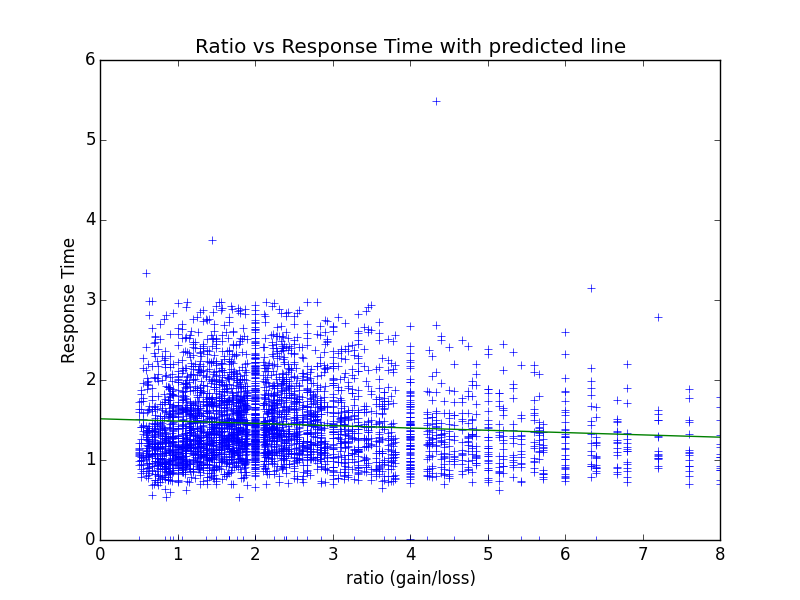
\includegraphics[scale=0.5]{../fig/lin/linear_regression.png}	 
\caption{Fitted Linear Regression line on respond time and ration of gain and loss}
\end{figure}


\subsubsection {Logistic Regression}
\noindent
 Logistic Regression is a statistical technique capable of predicting a binary outcome. Since, 
in this data, the researchers classify the decision to gamble as \'1\' or \'0\' otherwise, we can 
use logistic regression technique to explain the subject's tendency to gamble or not based on 
the condition of the gain and loss amount given in the process of experiment. Our goal is to 
identify the how gain and loss amount influence each subject's response. To do this, we use 
the statsmodels Logit function. We specify the response column in the behavior txt file as the 
one containing the variable we're trying to explain and the gain and loss columns as the predictor
 variables. After plotting the results on the plot, we were able to see some interesting behaviors
  of some subjects. As you see from the plot, Subject 1 is in general more risk seeking: as long 
  as the gain amount is large enough as 20 dollars, he decides to gamble. However, Subject 3 shows
   the opposite behavior: she does not participate in the gamble when her loss amount is higher 
   than 10 dollars no matter what the gain amount is. (To see the overall behaviors from all subjects,
    see the appendix) Overall, we could see that the logistic regression line fits well on the 
    border between the decision to gamble and not gamble. 

\begin{figure}[H] 
\centering 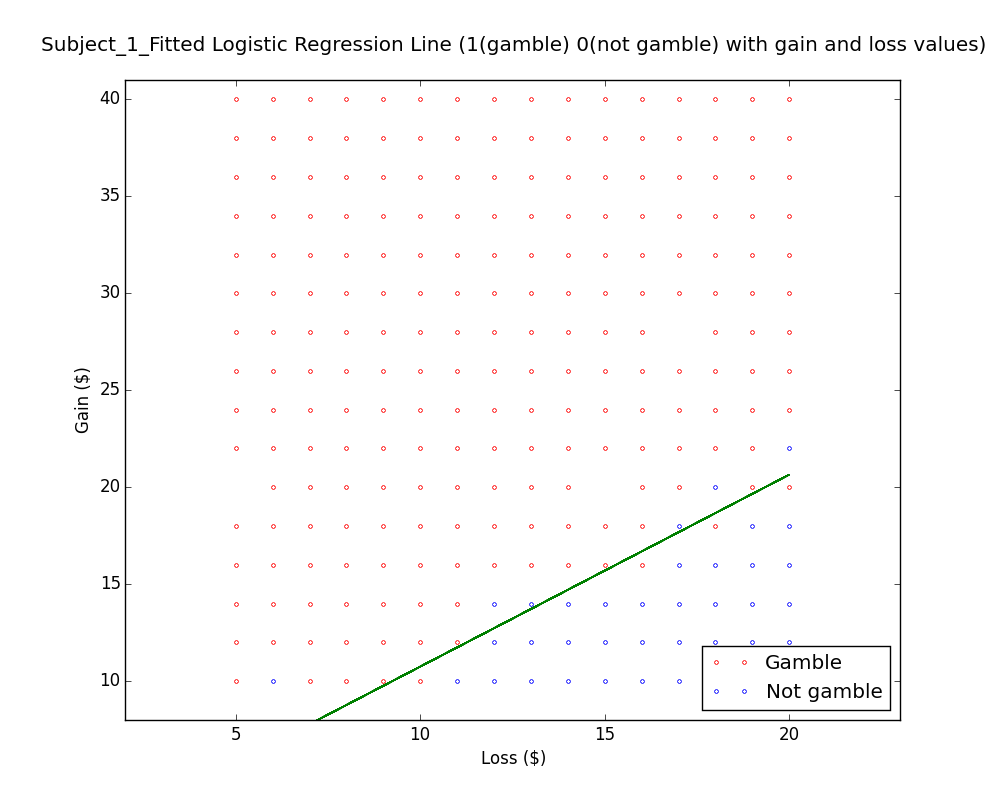
\includegraphics[scale=0.35]{../fig/log_reg_behav/log_regression_1.png}	 
\caption{Fitted Logistic Regression line on subject 1’s behavior data (predictors\: gain, loss)}
\end{figure} 

\begin{figure}[H] 
\centering 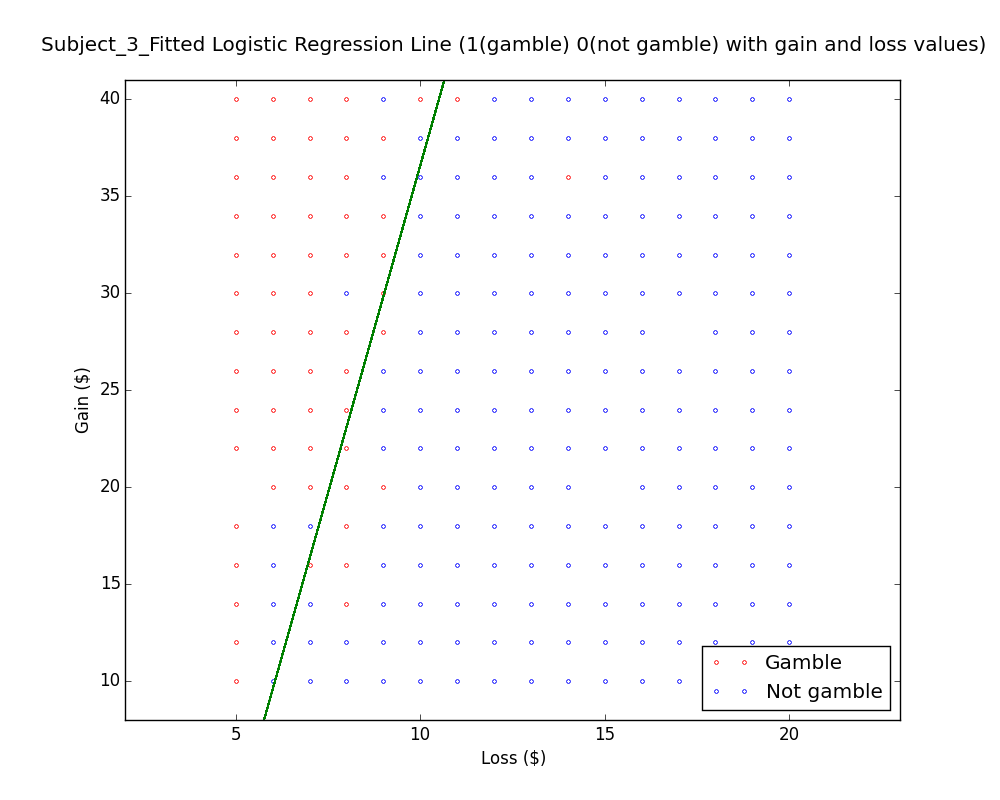
\includegraphics[scale=0.35]{../fig/log_reg_behav/log_regression_3.png}	 
\caption{Fitted Logistic Regression line on subject 3’s behavior data (predictors\: gain, loss)}
\end{figure} 


\subsection {Results}
The paper illustrates as \"people typically reject gambles that offer 
a 50/50 chance of gaining or losing money, unless the amount that could be gained is at 
least twice the amount that could be lost (Sabrina).\" In the experiment, the given gain 
and loss amount ratio to each subject is around 2 to 1. This refers subjects would not mere
ly show risk averse behavior every trial. We could confirm this trend by observing the p
lots. We are hard to tell whether subjects are risk averse or not.





